
\section{Inference with known exposure status}

\paragraph{}Using our simulated noisy serological data, this section will show how to infer several latent processes, including the population-level antibody kinetics, the correlate of protection, and the individual-level infectious state. We show simulation recovery in a simplified framework where we assume the exposure status of every individual (represented by vector $\mathbf{E}$) and exposure time (represented by vector $\mathbf{E^\tau}$) is known. Though knowing this information is rarely feasible in practice, working through this example will help explain how the inference on the fitted parameters, $\theta$ (describing the COP and antibody kinetics), and infection state, $\mathbf{Z}$, work without needing to describe the more complex inference using RJ-MCMC. 

\subsection{Mathematical representation of framework}

\paragraph{}Let the binary vector $\mathbf{E} = \{ E_1, E_2, \dots, E_M\}$, represent the exposure status of each individual $j$ where $E_j = 0$ is not exposed and $E_j = 1$ is exposed and let $n_\mathbf{E} = \sum_{j = 1}^ME_j$ be the number of exposed individuals. Then, let the vectors $\mathbf{E}^\tau = \{E_1^\tau, E_2^\tau, \dots, E^\tau_{n_\mathbf{E}}\}$ and $\mathbf{Z} = \{Z_1, Z_2^, \dots, Z_{n_\mathbf{E}}\}$ be the timing of the exposure and the infection state respectively for each individual which is exposed. The infection state is a binary vector where $Z_j = 0$ is not infected, and $Z_j = 1$ is infected. Let $Y_{j, t} \in \mathbf{Y}$ represent the dataset of titre values for individual $j$ and at time $t$. 

\paragraph{}We define several functions to help us calculate the likelihood of our model. First, we define a biologically-informed function that models the latent antibody titre at time $t$ for individual $j$, $A_{j,t}$, given their infection status $Z_j$ and timing of exposure $E_j^\tau$. If a person is not infected, their starting titre value ($Y^0_i$) remains unchanged. If the person is infected, their titre remains unchanged until the point of infection, after which they follow the kinetic function in \textbf{Equation~\ref{eq_ab}}. Although our simulated data has individual-level trajectories that vary from a population mean according to our variability level (10\%, 30\%, 50\%), here we estimate the population-level antibody kinetics function, averaging over the individual-level antibody kinetics. The deterministic function for calculating the latent antibody titre at time $t$ for individual $j$, $A_{j,t}$ depends on the timing of exposure for the individual, so $A_{j,t}$ is given by

\begin{equation}
\label{eq:ll_abkin}
A_{j,t}  = g_{ab}( Z_j,  E_j^\tau, \theta_{ab}, Y^0_j) = 
	\begin{cases}
	Y^0_j + f_{ab}(t - E_j^\tau, \theta_{ab}, Y^0_j),  & \text{If $Z_j = 1$, $E_j = 1$, and $t > E_j^\tau$} \\
	Y^0_j, & \text{Otherwise} \\ 
	\end{cases}
\end{equation}

Where $\theta_{ab} = \{a, b, c\}$. Second, we define a likelihood function for the correlate of protection. For an individual $j$, with $E_j = 1$, the correlate of protection given exposure at time $t$ with titre value $A_{j, t}$, is assumed to follow a Bernoulli distribution with the probability is given by \textbf{Equation~\ref{eq_cop}}. The PDF of this likelihood is given by \textbf{Equation~\ref{eq:ll_cop}}.

\begin{equation}
\label{eq:ll_cop}
P_{cop}(Z_j \mid Y_{j}^0, \theta_{cop} ) =  f_{cop}(Y_{j}^0,  \theta_{cop})^{Z_j}(1- f_{cop}(Y_{j}^0,  \theta_{cop} ))^{1-Z_j}
\end{equation}

\paragraph{}where $\theta_{cop} = \{\beta_0, \beta_1\}$. Finally, we define an observational model to capture variability between hosts and measurement error. Given $A_{j,t}$ and the serological antibody data at the same time point is given by $Y_{j, t}$, we assume the measurement error follows a normal distribution with a PDF given by \textbf{Equation~\ref{eq:ll_obs}}.

\begin{equation}
\label{eq:ll_obs}
P_{obs}(Y_{j,t} \mid A_{j,t}, \sigma) = \frac{1}{\sigma \sqrt{2\pi}} \, e^{-\left(\frac{(Y_{j,t} - A_{j,t})^2}{2\sigma^2}\right)}
\end{equation}

Let $\theta = \{a, b, c, \beta_0, \beta_1, \sigma\}$ be the set of continuous parameters which are to be fitted in the model. 

\subsection{Posterior distribution via Bayes rule}

We have two different likelihoods depending on whether an individual is exposed ($E_j = 1$) or not ($E_j = 0$).

\subsubsection{Likelihood for an non-exposed individual $E_j = 0$} 
In this case, the value of the timing of exposure and infection status is not applicable and thus not inferred. The likelihood for individual $j$ with serological samples taken at times $t\in T_j$ is therefore equivalent to:
\begin{equation}
\label{ll:1E0}
L_{E_j = 0}(Y_{j}| \theta) = \prod_{t \in T_j}P_{obs}(Y_{j,t}|Y^0_{j}, \sigma)
\end{equation}
as $A_{j.t} = Y^0_{j}$ for all $t$.


\subsubsection{Likelihood for an exposed individual $E_j = 1$}
In this case, the infection status is determined by the correlate of the protection likelihood ($P_{cop}$) and the antibody kinetics function. The likelihood for this individual with serological samples taken at times $t\in T_j$ and infection time $E^\tau_j$ is therefore equivalent to:

\begin{equation}
\label{ll:1E1}
L_{E_j = 1}(Y_{j}| Z_j, \theta) = \prod_{t \in T_j}P_{obs}(Y_{j,t}| A_{j,t}, \sigma)P_{cop}(Z_j \mid Y_{j}^0, \theta_{cop})
\end{equation}

where $A_{j,t} = g_{ab}( Z_j,  E_j^\tau, \theta_{ab}, Y^0_j)$.


\subsubsection{Total likelihood}

If $\mathbf{E_0}$ and $\mathbf{E_1}$ are vectors representing the set of individuals who are not exposed and exposed, respectively. Then, the total likelihood can be written 

\begin{equation}
L(\mathbf{Y} | \mathbf{Z}, \theta) = \prod_{j \in \mathbf{E_0}}L_{E_j = 0}(Y_{j}| \theta) \prod_{j \in \mathbf{E_1}}L_{E_j = 1}(Y_{j}| Z_j, \theta) 
\end{equation}


\subsubsection{Prior distributions}

\paragraph{}We choose prior distributions for each parameter \pi($\theta$). \textbf{Table~\ref{tab:priorsA}} summarises the chosen priors with their support. 

\begin{table}[ht]
    \centering
    \begin{tabular}{|l|l|l|}
        \hline
        \textbf{Parameter} & \textbf{Prior ($\pi$)} & \textbf{Support ($\mathcal{S}$)} \\
        \hline
        a & $\mathcal{N}(1.5, 0.5)$ & $[0.5, 4]$ \\
        \hline
        b & $\mathcal{N}(0.3, 0.05)$ & $[0, 1]$ \\
        \hline
        c & $\mathcal{U}(0, 4)$ & $[0, 4]$ \\
        \hline
        $\beta_0$ & $\mathcal{U}(-10, 10)$ & $[-10, 10]$ \\
        \hline
        $\beta_1$ & $\mathcal{U}(-10, 10)$ & $[-10, 10]$ \\
        \hline
        $\sigma$ &  $\mathcal{U}(0.01, 1)$ & $[0.01, 1]$ \\
        \hline
    \end{tabular}
    \caption{Table with Headers: Parameter, Prior, and Support}
    \label{tab:priorsA}
\end{table}

\paragraph{}We also choose the prior for the number of infections $n_\mathbf{Z}$ given the number of exposed individuals $n_\mathbf{E}$ to be a Beta Binomial distribution: $\pi(\mathbf{Z}) = \text{BetaBinomial}(n_\mathbf{Z} | n_\mathbf{E}, 1, 1)$. Choosing this prior prevents any implicit priors that might rise from products of Bernoulli trials\cite{Hay2020-pr} as $\text{BetaBinomial}(n_\mathbf{Z} | n_\mathbf{E}, 1, 1) = 1 / n_\mathbf{E}$ for all $0 \leq n_\mathbf{Z} \leq n_\mathbf{E}$. 

% Note important for this changes inference
% 

\subsubsection{Posterior distributions}

\paragraph{}Bayes' rule stipulates that the product of the prior distribution and likelihood is proportional to the posterior distribution; we can use this rule to approximate the posterior for use in the metropolis algorithm. Specifically 

\begin{equation}
\label{eq:bayes}
P(\theta, \mathbf{Z} | \mathbf{Y}) \propto \mathcal{L}(\mathbf{Y} | \mathbf{Z}, \theta)\pi(\theta)\pi(\mathbf{Z})
\end{equation}


\subsection{Metropolis-Hastings for serological inference with known exposure }

\paragraph{}An overview of the Metropolis-Hasting algorithm is in \textbf{Appendix Section~\ref{sec:mh1}}. In this section, we define the proposal distribution required to sample from \textbf{Equation~\ref{eq:bayes}}, which infers $\theta$, and infection statuses ${Z_j} \in \mathbf{Z}$, for $1 \leq j \leq M$ individuals. A schematic showing the relationship between the state variables and likelihood functions is given in \textbf{Figure~\ref{fig:sch_B}}.

\begin{figure}[H]
    \centering
    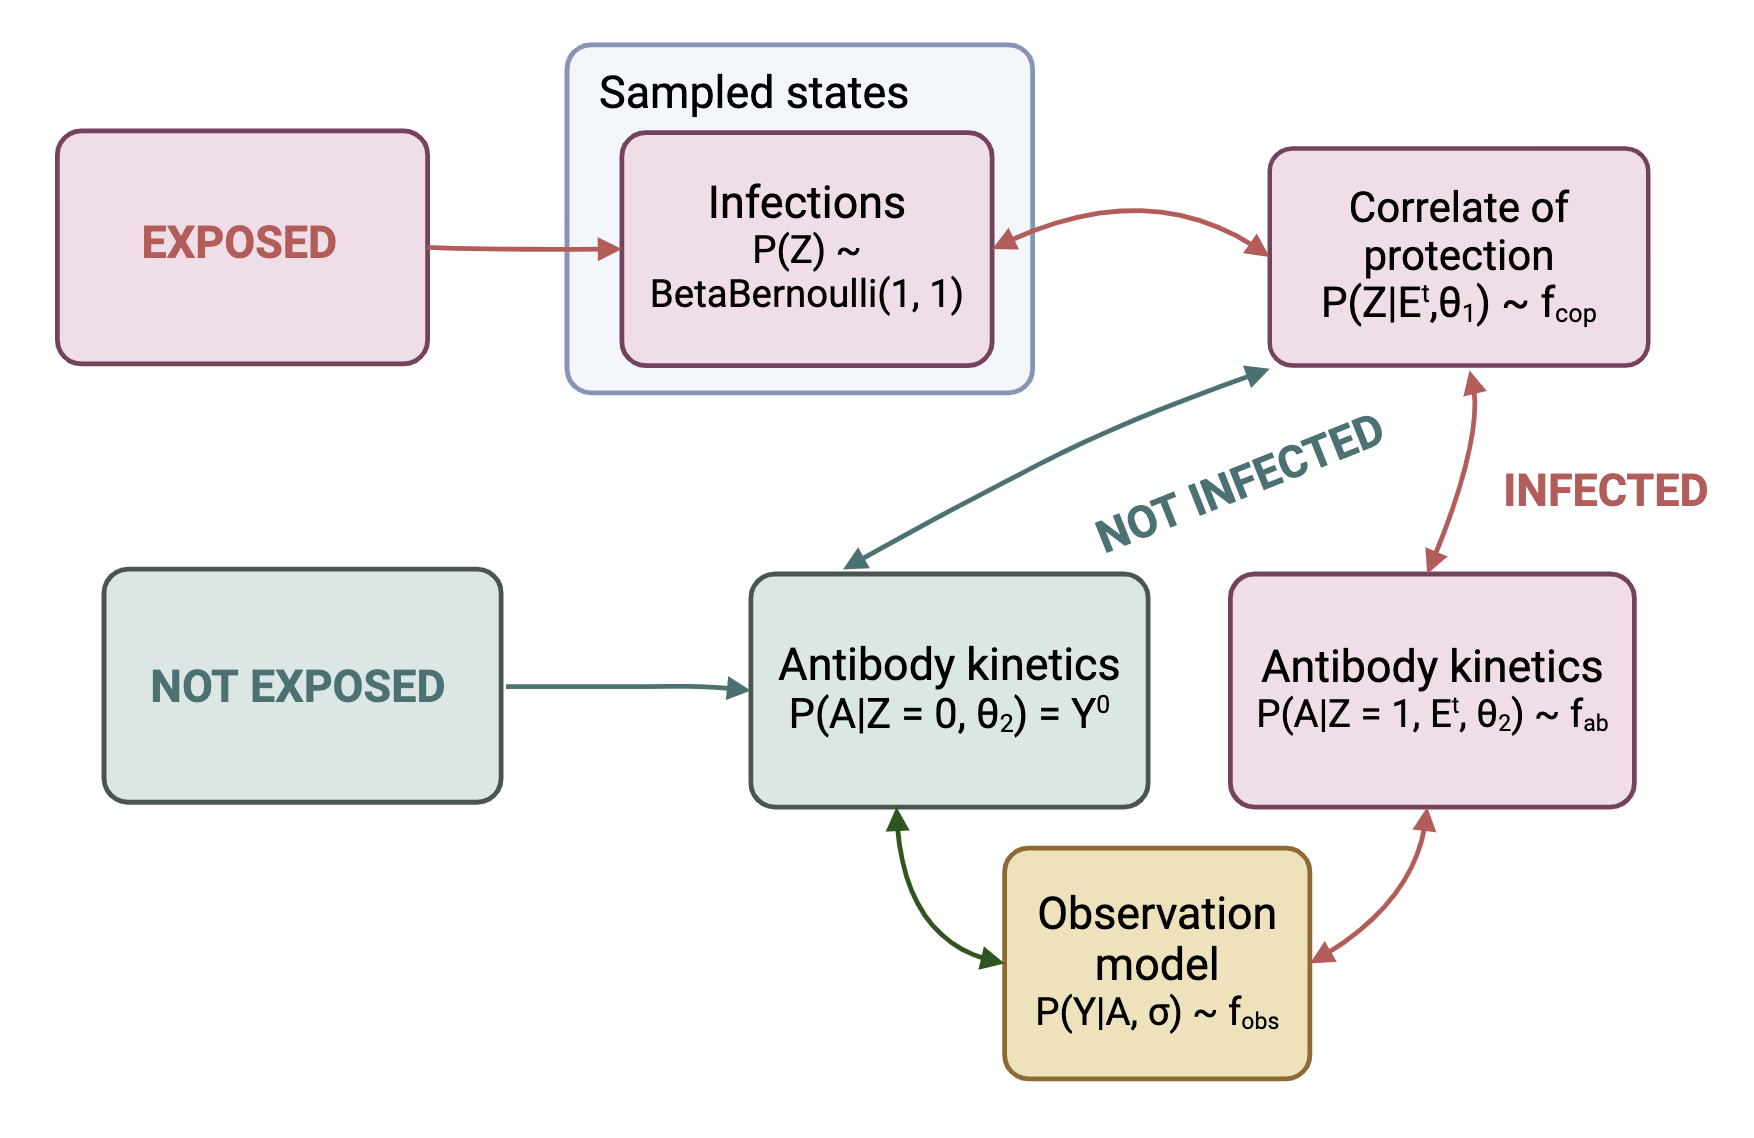
\includegraphics[width=1\textwidth]{sections/s3_known_exp/figs/sch_B.png}     \caption{Schematic showing the relationship between the sampled states for $Z$ and the likelihood functions.\label{fig:sch_B}}
\end{figure}


\paragraph{}We define independent proposal distribution for $\theta$ and $\mathbf{Z}$,  such that $Q(\cdot | \theta, \mathbf{Z}) = q_\theta(\cdot |\theta)q_Z(\cdot |\mathbf{Z})$. At Markov chain step $i$, we have a value of the parameter space, $\theta^{(i)}$, and propose a new set of parameters $\theta'$ via the proposal distribution $\theta \sim q_\theta(\cdot | \theta^{(i)}, \psi^{(i)}_{adapt})$. This proposal is a multivariate normal distribution with an adaptive covariance matrix, which is defined by the set of parameters $\psi^{(i)}_{adapt}$, which are updated at each time step.\cite{Roberts2012-ju, Andrieu2008-yx} (see \textbf{Appendix~\ref{app:adapt}}). For $\mathbf{Z}$, we propose a new infection state $\mathbf{Z}'$ by selecting an exposed individual $j$, which has infection status $Z_j^{(i)}$ at step $i$ of the current Markov chain, and sample a proposal value for their infection status $Z_j'$ by the proposal distribution for $Z_j' \sim q_Z(\cdot | Z^{(i)}_j)= \text{Bernoulli(0.5)}$. Therefore the proposal for $q_Z(\mathbf{Z}'|\mathbf{Z}) = 1/n_\mathbf{E}0.5$ for all $j$. Both of these proposals $q_\theta\left(\theta' | \theta^{(i)}, \psi^{(i)}_{adapt}\right)$, $q_Z(\mathbf{Z}'|\mathbf{Z})$ are symmetric and thus cancel out the acceptance ratio (\textbf{Equation~\ref{eq:alpha}}). Further, the prior distribution $\pi(\mathbf{Z}) = 1 / n_\mathbf{E}$ for all $0 \leq n_\mathbf{Z} \leq n_\mathbf{E}$, and thus also cancels out in the acceptance ratio, therefore we need only calculate: $P(\theta, \mathbf{Z} | \mathbf{Y}) \propto \mathcal{L}(\mathbf{Y} | \mathbf{Z}, \theta)\pi(\theta)$. \textbf{Algorithm~\ref{alg:metropolis_hastings_inf}} is a Metropolis-Hasting algorithm which samples from this proposal.

\begin{algorithm}[H]
\caption{Metropolis-Hastings Algorithm for antibody kinetics and infection inference}
\label{alg:metropolis_hastings_inf}
\begin{algorithmic}[1]
    \State Initialize the chain with an initial state $\theta^{(0)}$ from the priors $\pi(\cdot)$ and $I^{(0)}_{j} \sim \text{Bernoulli(0.5)}$ for all $1 \leq j \leq M$ individuals to intialise $\mathbf{Z}^{(0)}$, and initialise $\psi^{(0)}_{adapt}$.
    \For{$i = 1$ to $N$}
        \State Generate a candidate state $\theta' \sim q_\theta\left(\theta^{(i)}, \psi^{(0)}_{adapt}\right)$
        \State Generate a candidate individual $j \in \mathbf{E_1} $, then a candidate state $Z_j \sim \text{Bernoulli(0.5)}$ to propose $\mathbf{Z}'$
        \State Compute the acceptance ratio:
        \[
        \alpha((\theta^{(i)}, \mathbf{Z}^{(i)}),( \theta',  \mathbf{Z}')) = \min\left(1, \frac{P(\theta', \mathbf{Z}'|\mathbf{Y})}{P(\theta^{(i)}, \mathbf{Z}^{(i)}|\mathbf{Y})} \right)
        \]
        \State Sample $u \sim \mathcal{U}(0, 1)$
        \If{$u \leq \alpha$}
            \State Accept the candidate state: $\theta^{(i+1)} \leftarrow \theta'$ and $\mathbf{Z}^{(i + 1)}  \leftarrow \mathbf{Z}'$
        \Else
            \State Reject the candidate state: $\theta^{(i+1)} \leftarrow \theta^{(i)}$ and $\mathbf{Z}^{(i + 1)}  \leftarrow \mathbf{Z}^{(i)} $
        \EndIf 
        \State Update $ \psi^{(i + 1)}_{adapt} \leftarrow \psi^{(i)}_{adapt}$
    \EndFor
\end{algorithmic} 
\end{algorithm}


\subsection{Implementation }
\paragraph{}  \textbf{Algorithm~\ref{alg:metropolis_hastings_inf}} is coded manually in R and C++ through Rcpp. We run the algorithm for four chains, each with 400,000 steps and 200,000 burn-in steps. The initial values for $\theta$ and $\mathbf{Z}$ are sampled from their prior distributions. We initialise the adaptive covariance by running with an identity matrix with each parameter scale according to 1,000 steps, then sample from the adaptive scheme (see \textbf{Appendix~\ref{app:adapt}}). We thin the posterior samples by taking one in every 100, leaving 2,000 posterior samples at the end of the sampling. The trace plots for each of the six models fits are given in \textbf{Appendix Figure~\ref{app_traceA}}.

\subsection{Simulation recovery }
\paragraph{} After running \textbf{Algorithm~\ref{alg:metropolis_hastings_inf}}, we plot the posterior samples, $\hat{\theta}$ and $\hat{\mathbf{Z}}$ and compare with the simulated parameters.

\subsubsection{Infection recovery}

\paragraph{}We assess the algorithm's ability to recover each individual's infection status in the study. Suppose the set posterior samples of the infection status for individual $j$ is given by $\hat{Z_j} $. In that case, we plot the expectation $\mathbb{E}[\hat{Z_j}]$ so we can assess the ability of the algorithm to recover the individual-level simulated infection status (\textbf{Figure~\ref{fit1:inf}}). All models except one recovered the infection status for all individuals and correctly estimated the number of individuals infected across the study. The COP with 50\% variability has one individual out of 200 misclassified, predicting this individual was not infected when it indeed was. 


\begin{figure}[H]
    \centering
    \begin{subfigure}{0.31\textwidth}
        \centering
        \includegraphics[width=\textwidth]{\myimagepath/outputs/fits/cesNoCOP_notd/knownExp/figs/obs_0.1/infection_recov.png}
        \caption{No COP, 10\% variability \label{fit1:infA}}
    \end{subfigure}
    \begin{subfigure}{0.31\textwidth}
        \centering
        \includegraphics[width=\textwidth]{\myimagepath/outputs/fits/cesNoCOP_notd/knownExp/figs/obs_0.3/infection_recov.png}
        \caption{No COP, 30\% variability \label{fit1:infB}}
    \end{subfigure}
    \begin{subfigure}{0.31\textwidth}
        \centering
        \includegraphics[width=\textwidth]{\myimagepath/outputs/fits/cesNoCOP_notd/knownExp/figs/obs_0.5/infection_recov.png}
        \caption{No COP, 50\% variability \label{fit1:infC}}
    \end{subfigure}
    
  \begin{subfigure}{0.31\textwidth}
        \centering
        \includegraphics[width=\textwidth]{\myimagepath/outputs/fits/cesCOP_notd/knownExp/figs/obs_0.1/infection_recov.png}
        \caption{ COP, 10\% variability \label{fit1:infD}}
    \end{subfigure}
    \begin{subfigure}{0.31\textwidth}
        \centering
        \includegraphics[width=\textwidth]{\myimagepath/outputs/fits/cesCOP_notd/knownExp/figs/obs_0.3/infection_recov.png}
        \caption{ COP, 30\% variability \label{fit1:infE}}
    \end{subfigure}
    \begin{subfigure}{0.31\textwidth}
        \centering
        \includegraphics[width=\textwidth]{\myimagepath/outputs/fits/cesCOP_notd/knownExp/figs/obs_0.5/infection_recov.png}
        \caption{ COP, 50\% variability \label{fit1:infF}}
    \end{subfigure}
    
    \caption{Simulation recovery of the individual infection status, $\mathbb{E}[\hat{Z_j}]$, for two COP models (top: No COP, bottom: logistic COP) and three different levels antibody kinetics variability (10\%, 30\%, 50\%) \label{fit1:inf}}
\end{figure}


\subsubsection{Correlate of protection}

\paragraph{}We next assess the ability of \textbf{Algorithm~\ref{alg:metropolis_hastings_inf}} to recover the correlate of protection function $f_{cop}(x, \hat{\theta}_{cop})$, where $x$ is the titre value at infection and where $\hat{\theta}_{cop} = \{\hat{\beta_0}, \hat{\beta_1}\}$ are the posterior samples for $\beta_0$ and $\beta_1$. We consider two COP models: COP model A, no correlate of protection, and COP model B, a logistic curve for COP. For Model A, we find that the COP curve is recovered, with the simulated line within a 95\% confidence interval of the posterior sample (\textbf{Figure~\ref{fit1:cop}}). For Model B, we also find the logistic shape of the COP is recovered in the posterior samples. The variability in the antibody kinetics seemed to have a negligible effect on the recoverability of the COP curve. 

\begin{figure}[H]

    \centering
    \begin{subfigure}{0.31\textwidth}
        \centering
        \includegraphics[width=\textwidth]{\myimagepath/outputs/fits/cesNoCOP_notd/knownExp/figs/obs_0.1/cop_recov.png}
        \caption{No COP, 10\% variability\label{fit1:copA}}
    \end{subfigure}
    \begin{subfigure}{0.31\textwidth}
        \centering
        \includegraphics[width=\textwidth]{\myimagepath/outputs/fits/cesNoCOP_notd/knownExp/figs/obs_0.3/cop_recov.png}
        \caption{No COP, 30\% variability \label{fit1:copB}}
    \end{subfigure}
    \begin{subfigure}{0.31\textwidth}
        \centering
        \includegraphics[width=\textwidth]{\myimagepath/outputs/fits/cesNoCOP_notd/knownExp/figs/obs_0.5/cop_recov.png}
        \caption{No COP, 50\% variability \label{fit1:copC}}
    \end{subfigure}
    
  \begin{subfigure}{0.31\textwidth}
        \centering
        \includegraphics[width=\textwidth]{\myimagepath/outputs/fits/cesCOP_notd/knownExp/figs/obs_0.1/cop_recov.png}
        \caption{ COP, 10\% variability\label{fit1:copD}}
    \end{subfigure}
    \begin{subfigure}{0.31\textwidth}
        \centering
        \includegraphics[width=\textwidth]{\myimagepath/outputs/fits/cesCOP_notd/knownExp/figs/obs_0.3/cop_recov.png}
        \caption{ COP, 30\% variability \label{fit1:copE}}
    \end{subfigure}
    \begin{subfigure}{0.31\textwidth}
        \centering
        \includegraphics[width=\textwidth]{\myimagepath/outputs/fits/cesCOP_notd/knownExp/figs/obs_0.5/cop_recov.png}
        \caption{ COP, 50\% variability \label{fit1:copF}}
    \end{subfigure}
    
    \caption{Simulation recovery of the COP function, with posterior samples plot  $f_{cop}(x, \hat{\theta}_{cop})$. We have two different COP models (top: No COP, bottom: logistic COP) and three different levels of antibody kinetics variability (10\%, 30\%, 50\%). \label{fit1:cop}}
    \end{figure}


\subsubsection{Antibody kinetics}

\paragraph{} \textbf{Algorithm~\ref{alg:metropolis_hastings_inf}} also recovers the simualted antibody kinetics. Let us plot $f_{ab}(s, \hat{a}, \hat{b}, \hat{c})$, the posterior predictive distribution for the antibody kinetic boosting, given posterior distributions  $\hat{a}, \hat{b}$, and $\hat{c}$. For the no COP model A, the antibody kinetics are recovered, though increasing variability weakens the accuracy of the recovered curves compared to the simulated when we compare the posterior distributions for $\hat{a}, \hat{b}, \hat{c}$ to the simulated value (\textbf{Figure~\ref{fit1:ab}}). For COP model B, there is a slight bias in the estimation for parameter $c$, being overestimated for variability levels $30\%$ and $50\%$. 

\begin{figure}[H]
    \centering
    \begin{subfigure}{0.31\textwidth}
        \centering
        \includegraphics[width=\textwidth]{\myimagepath/outputs/fits/cesNoCOP_notd/knownExp/figs/obs_0.1/ab_kinetics_recov.png}
        \caption{No COP, 10\% variability}
    \end{subfigure}
    \begin{subfigure}{0.31\textwidth}
        \centering
        \includegraphics[width=\textwidth]{\myimagepath/outputs/fits/cesNoCOP_notd/knownExp/figs/obs_0.3/ab_kinetics_recov.png}
        \caption{No COP, 30\% variability}
    \end{subfigure}
    \begin{subfigure}{0.31\textwidth}
        \centering
        \includegraphics[width=\textwidth]{\myimagepath/outputs/fits/cesNoCOP_notd/knownExp/figs/obs_0.5/ab_kinetics_recov.png}
        \caption{No COP, 50\% variability}
    \end{subfigure}
    
  \begin{subfigure}{0.31\textwidth}
        \centering
        \includegraphics[width=\textwidth]{\myimagepath/outputs/fits/cesCOP_notd/knownExp/figs/obs_0.1/ab_kinetics_recov.png}
        \caption{ COP, 10\% variability}
    \end{subfigure}
    \begin{subfigure}{0.31\textwidth}
        \centering
        \includegraphics[width=\textwidth]{\myimagepath/outputs/fits/cesCOP_notd/knownExp/figs/obs_0.3/ab_kinetics_recov.png}
        \caption{ COP, 30\% variability}
    \end{subfigure}
    \begin{subfigure}{0.31\textwidth}
        \centering
        \includegraphics[width=\textwidth]{\myimagepath/outputs/fits/cesCOP_notd/knownExp/figs/obs_0.5/ab_kinetics_recov.png}
        \caption{ COP, 50\% variability}
    \end{subfigure}
    
    \caption{Simulation recovery of the antibody kinetics function with posterior samples plot $f_{ab}(s, \hat{a}, \hat{b}, \hat{c})$. We have two different COP models (top: No COP, bottom: logistic COP) and three different levels of antibody kinetics variability (10\%, 30\%, 50\%). \label{fit1:ab}
}

\end{figure}

% JH: I guess it's hard to assess from just one simulation-recovery experiment. but looks like the waning rate estimates are biased in the no CoP case and alpha is biased in the CoP case. Any thoughts on why?
% One thing which doesn't come through obviously is that you simulate with random effects on the antibody kinetics parameters, but are fitting a model assuming everyone has the same kinetics parameters, right? I think that needs to be mentioned clearly.
% Looking again, similarly, it's not clear that you are plotting 3 quite different things:
% 1. The true mean value of each parameter
% 2. The distribution of individual parameter values
% 3. The estimated posterior distribution for the mean parameter value.
% I think what's confusing is the grey distribution and red distribution being shown alongside each other, and they are quite different things


